\section{Sensorik und Sicherheitstechnik \textcolor{gray}{(Elena Widmann)}}

\subsection{Aufgabenstellung}

\subsection{Sensorik}

\subsubsection{Endschalter}
Beim Verplanen der Endschalter ist zwischen Software- und Hardware-Endschalter zu unterscheiden. Die Software-Endschalter begrenzen den Arbeitsbereich der Achse und sollten innerhalb des Bereichs der Hardware-Endschalter parametriert werden. Ihre Positionen werden direkt im Siemens TIA-Portal eingestellt und können falls notwendig einfach auf die aktuelle Geschwindigkeit angepasst werden. Werden die Software-Endschalter angefahren, wird der Technologiealarm 533 ausgelöst, und die Dynamikwerte werden gestoppt, das Technologieobjekt bleibt hierbei freigegeben. Werden sie jedoch überfahren wird das Technologieobjekt gesperrt. \\
Die Hardware-Endschalter begrenzen den maximal zulässigen Verfahrensbereich der Achse. Bei ihnen wird nicht unterschieden, ob die Endschalter angefahren oder überfahren werden. Beim Anfahren der Schalter wird der Technologiealarm 531 ausgelöst. Er sperrt das Technologieobjekt und muss, bevor der Auslösebereich der Hardware-Endschalter wieder verlassen werden kann, quittiert werden. \cite{axis_manual}\\
Auf jeder der drei Achsen vom AFSS und auf dem Querförderer müssen Hardware-Endschalter montiert werden. Die Auswahl begrenzte sich hierbei auf die uns zur Verfügung gestellten Sensoren, welche unter Berücksichtigung ihrer Funktion auf den verschiedenen Positionen eingebaut werden.

\paragraph{Positionsschalter mit Rollhebel} \mbox{}\\
An der x-Achse werden als Hardware-Endschalter Positionsschalter mit Rollhebel verwendet (siehe Abb. \ref{roll_sens}). Davon besitzen drei jeweils einem Öffner- und einen Schließerkontakt \cite{schmersal_3}, wohingegen einer der Endschalter aus zwei Öffnerkontakten besteht. \cite{schmersal_1} Um Einheitlich zu bleiben und da es sicherheitstechnisch auch von Vorteil ist (Drahtbruchsicherheit) verwenden wir jeweils einen der Öffnerkontakte der Endschalter. Zum Schalten des Rollhebels der Positionsschalter müssen auf dem x-Schlitten der oberen sowie unteren x-Achse Auslöser angebracht werden. Diese befinden sich mittig auf der Seite der Sensoren und gleichen einem vom Schlitten abstehenden Arm, welcher sich aus gestapelten, mit dem Lasercutter gefertigten, Teilen zusammensetzt.

\paragraph{Induktive Endschalter} \mbox{}\\
Als Hardware-Endschalter an der y-Achse werden induktive Sensoren verwendet (siehe Abb. \ref{ind_sens}). Sie funktionieren so, dass durch eine Spule ein Magenetfeld erzeugt wird, welches dann in einem sich dem Sensor frontseitig nähernden elektrisch leitendem Material Wirbelströme erzeugt. Dadurch verändert sich das Magnetfeld und die Kontakte des induktive Sensors werden über einen Schmitt-Trigger geschaltet. Die Sensoren besitzen jeweils einen Öffner- und einen Schließerkontakt, wir verwenden jedoch ersteres um Drahtbruchsicherheit zu gewährleisten. Damit die induktiven Sensoren korrekt auslösen können, müssen auf dem Shuttle der y-Achse elektrisch leitende Gegenstücke, in unserem Fall aus Metall, angebracht werden.

\paragraph{Endtaster} \mbox{}\\
An der z-Achse und am Querförderer werden mechanische Endtaster als Endschalter verwendet. Auf einem Endtaster befindet sich ein Schließerkontakt in Form eines Tasters, welcher durch anfahren geschalten wird (siehe Abb. \ref{tast_sens}). Zum Betätigen der Taster müssen sich Auslöser auf dem Shuttle und den Seiten der Querfördererstation befinden.\\

\begin{figure}[H]
    \centering
    \begin{subfigure}{.3\textwidth}
        \centering
        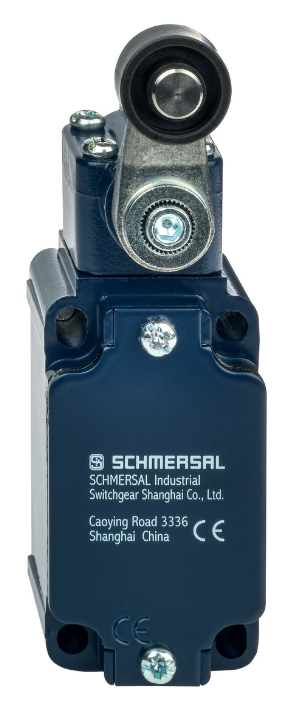
\includegraphics[width=0.5\textwidth]{Sensors/Rollendschalter.png}
        \caption{Rollendschalter \cite{schmersal_pic}}
        \label{roll_sens}
    \end{subfigure}%
    \begin{subfigure}{.3\textwidth}
        \centering
        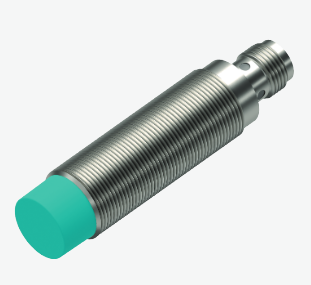
\includegraphics[width=1\textwidth]{Sensors/Induktiver_Sensor.png}
        \caption{Induktiver Sensor \cite{induktiv_sensor}}
        \label{ind_sens}
    \end{subfigure}%
    \begin{subfigure}{.3\textwidth}
        \centering
        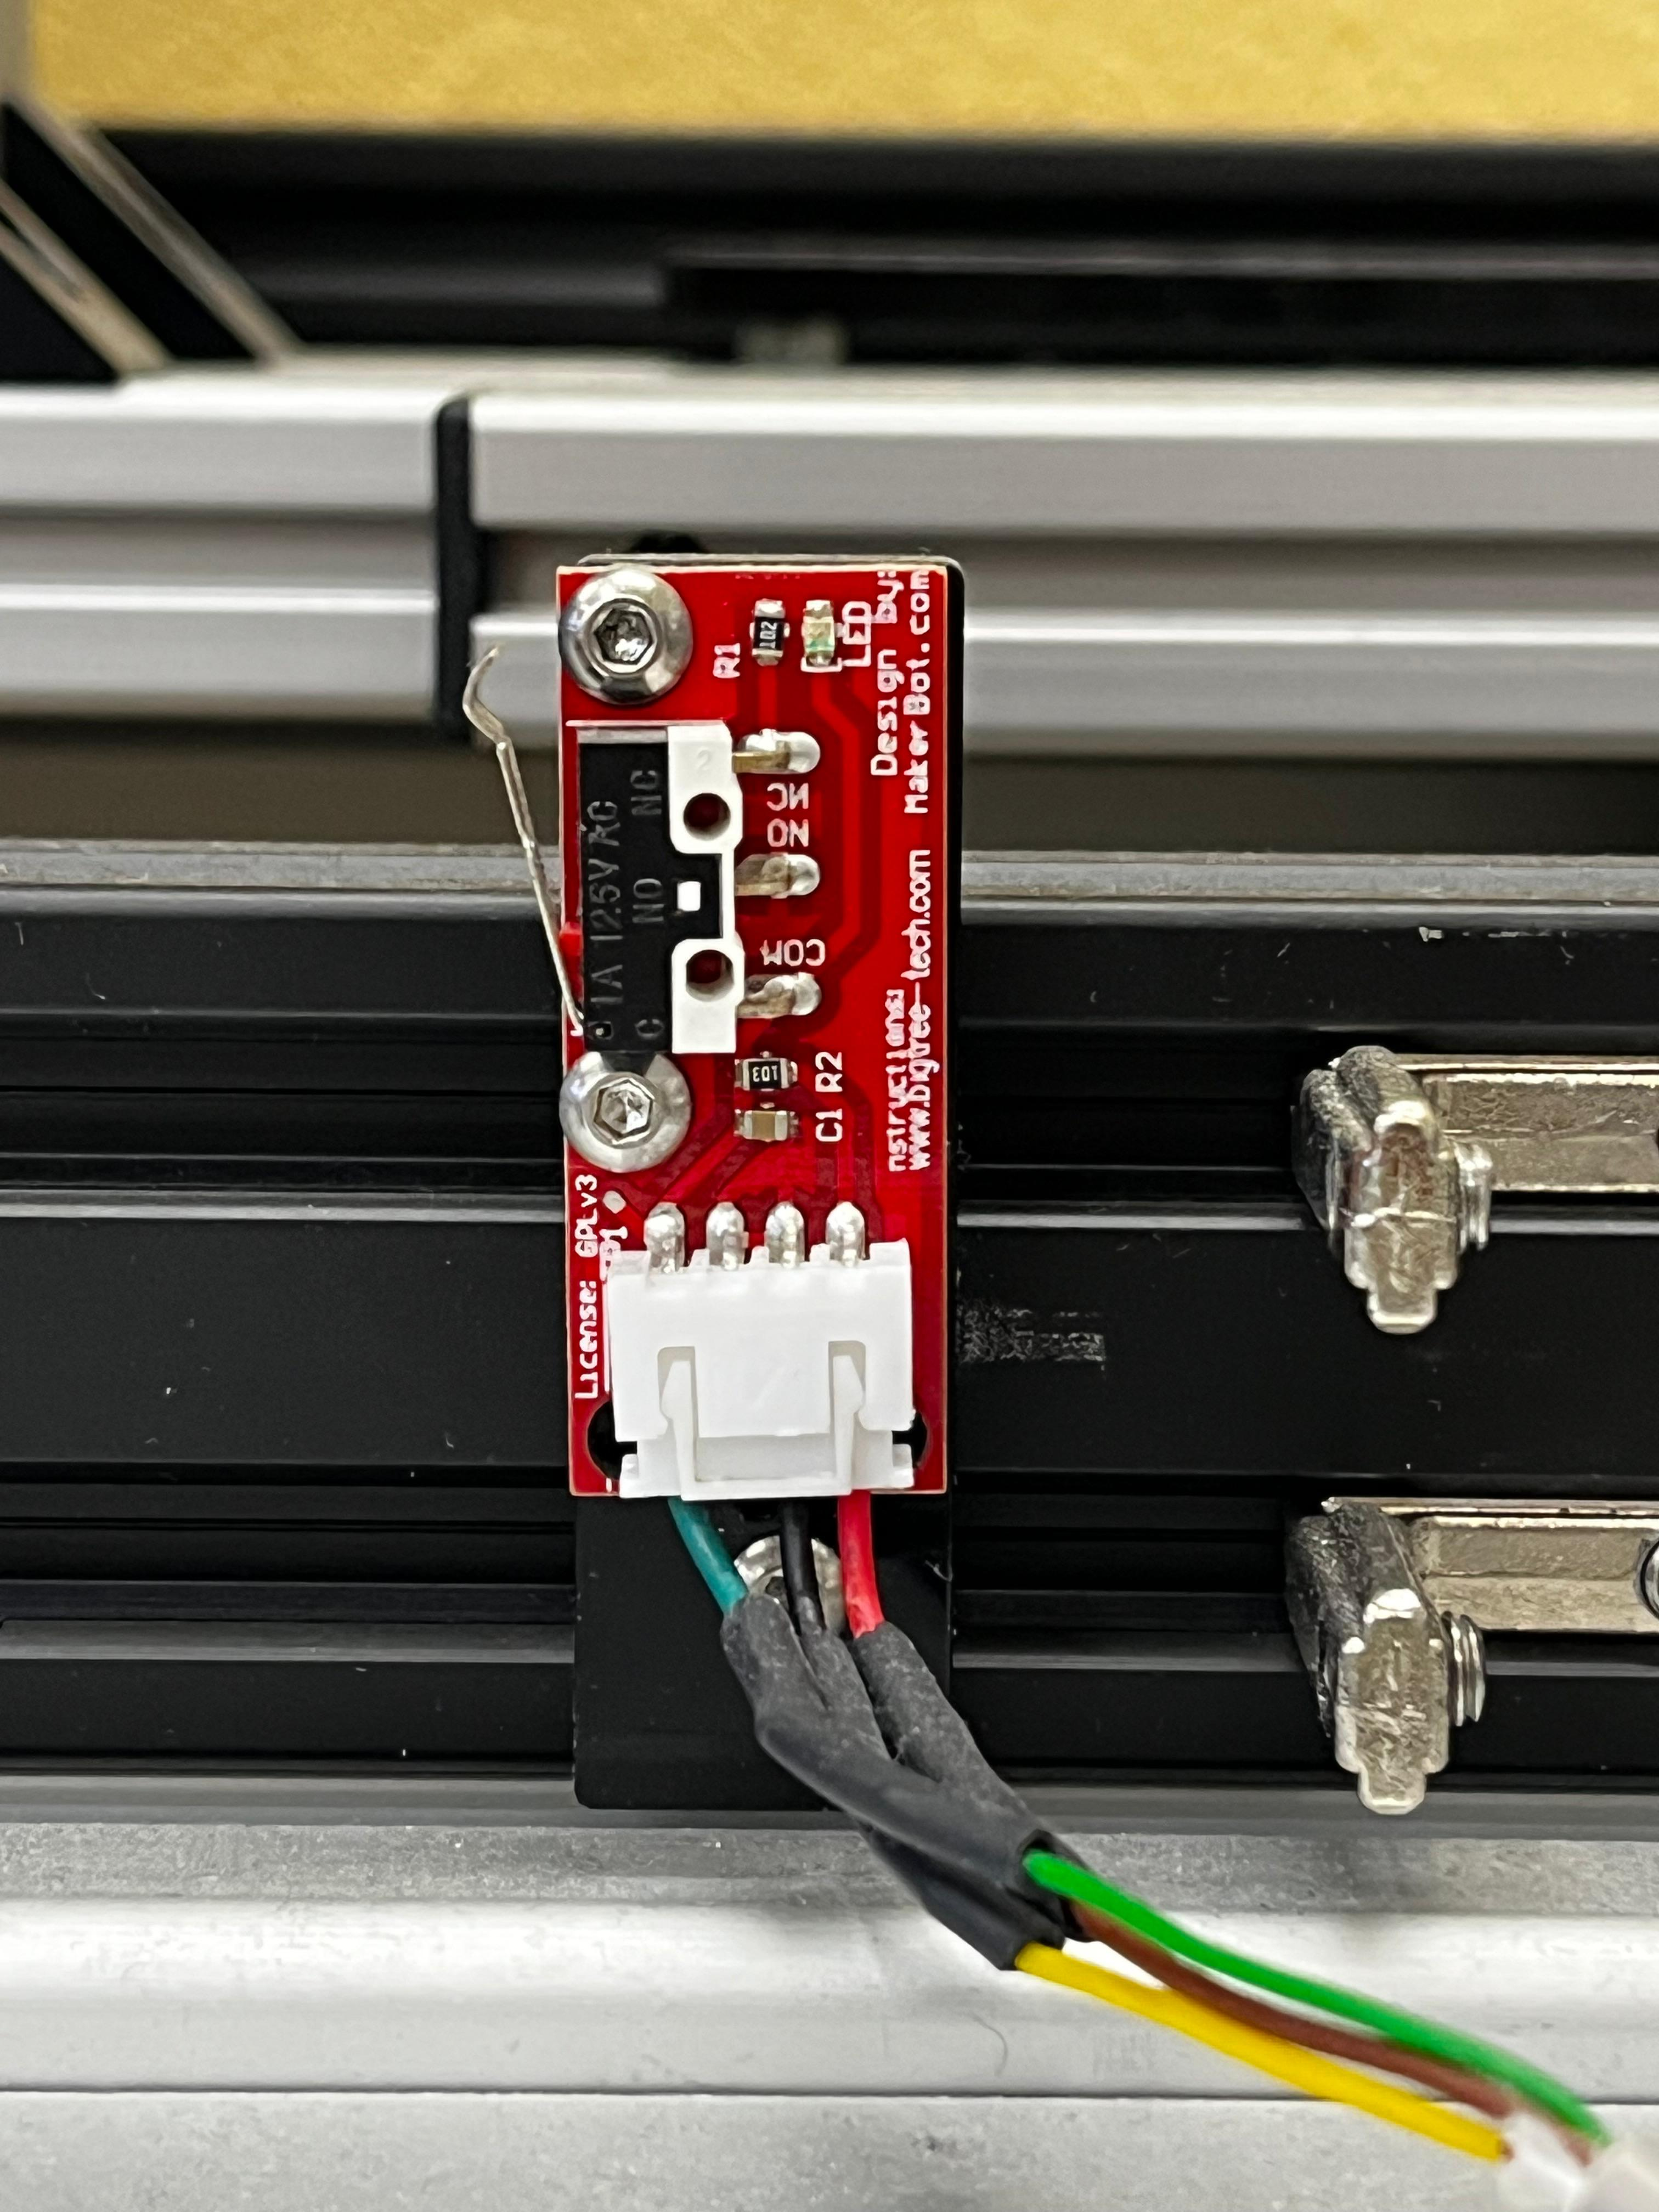
\includegraphics[width=0.9\textwidth]{Sensors/Endtaster.jpg}
        \caption{Endtaster}
        \label{tast_sens}
    \end{subfigure}
    \caption{Endschalter}
    \label{ulr}
\end{figure}

\subsubsection{Referenztaster}
Um die Motoren auf die richtige Position fahren zu können, müssen diese an allen drei Achsen und am Querförderer referenziert werden. Somit wird verhindert, dass auch bei einem Neustart des Systems sich die Koordinaten der Positionen, auf denen sich die Bauteilboxen befinden, nicht verändern und es zu keiner Kollision zwischen Shuttle und einer Box kommt.\\
Zum Referenzieren müssen Sensoren an den Achsen und am Querförderer angebracht werden, welchen den jeweiligen Nullpunkt angeben. Hierfür werden Opto Interrupter verwendet, da diese einfach durch anfahren ausgelöst werden können. In einem Opto Interrupter befindet sich eine LED, dessen Lichtstrahl auf einen Photo Transistor trifft. Dieser schaltet daraufhin durch und es liegt eine Spannung am Emitter an. Wird jetzt jedoch der Lichtstrahl der LED unterbrochen, sperrt der Transistor und es fließt kein Strom. Bei der SPS-Programmierung ist daher zu beachten, dass sich der Ausgang des Sensors im nicht geschalteten Zustand auf HIGH befindet. Wird der Lichtstrahl jedoch unterbrochen, liegt am Sensorausgang keine Spannung an und der Eingang der SPS erhält ein LOW Signal.\\
In unserem Fall werden TP808 zum Referenzieren verwendet. Hierbei ist zu beachten, dass die sich darin befindende Diode nur mit einer maximalen Flussspannung von 1.35V betrieben werden darf.\cite{TP808} Da die Opto Interrupter jedoch über ASi-Bus mit der SPS verbunden werden, welche eine Spannung von 24V liefert, muss eine eigene Platine entworfen und gelötet werden, um das Bauteil nicht mit einer zu hohen Betriebsspannung zu zerstören. Hierfür wird die Software Fusion360 verwendet, welche das Designen von Leiterplatten ermöglicht. Hergestellt werden diese dann durch unsere eigene schulinterne Leiterplattenfertigung.

\paragraph{Schaltungsentwurf} \mbox{}\\
Die Schaltung sollte so konzipiert sein, dass keines der involvierten Bauteile über längeren Normalbetrieb oder durch kurzzeitige hohe Ströme bzw. Spannungen, beschädigt wird. Das Ziel ist, die korrekte Funktion des Opto Interrupters auch zukünftig noch sicher stellen zu können. Dafür ist besonders wichtig auf dessen elektrische Eigenschaften zu achten, welche im Datenblatt zu finden sind.\\
Im Opto Interrupter befindet sich eine LED mit einer maximalen Durchlassspannung von 1.35V. und einer typischen von 1.2V. Um diese nicht mit den vollen 24V zu überlasten muss ein Vorwiderstand eingebaut werden. Dieser wird durch das ohm'sche Gesetz berechnet mit 

\paragraph{Platinenentwurf und -herstellung} \mbox{}\\

\begin{figure}[H]
    \centering
    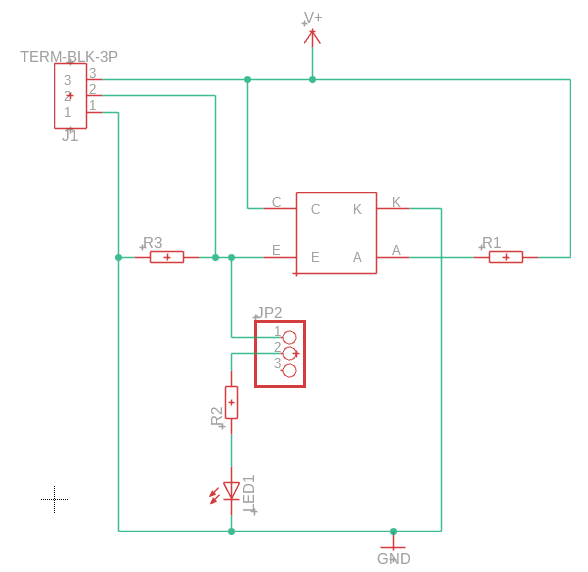
\includegraphics[width=0.6\textwidth]{Sensors/Ref_Schaltplan.png}
    \caption{Schaltplan Referenzplatine}
    \label{Ref_Schaltplan}
\end{figure}

\begin{figure}[H]
    \centering
    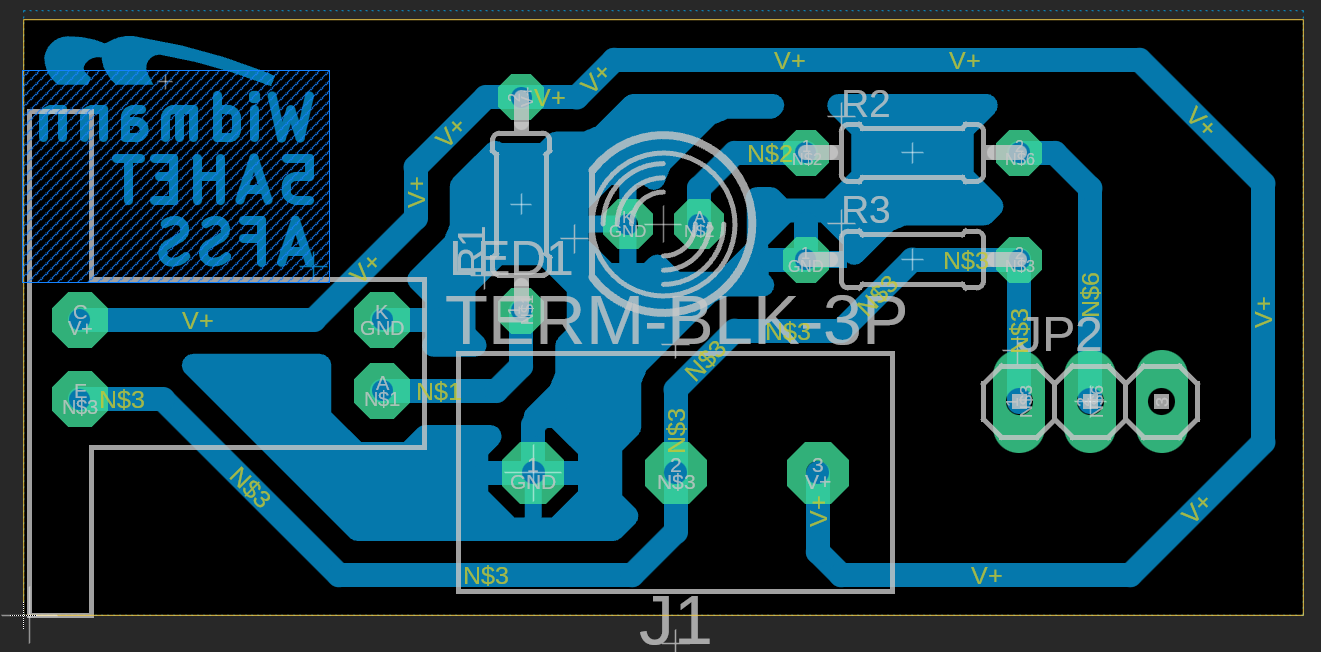
\includegraphics[width=0.7\textwidth]{Sensors/Ref_Leiterplattenplan.png}
    \caption{Leiterplattenplan Referenzplatine}
    \label{Ref_LPPlan}
\end{figure}

Damit während eines Referenziervorgangs der Lichtstrahl der LED unterbrochen wird und der Referenztaster auslöst, müssen auch hier wieder Auslösevorrichtungen an den x-Schlitten, am Shuttle und auf den Seiten der Querfördererstation angebracht werden.

\subsubsection{Lichttaster}

\subsubsection{Barcode-Scanner}

\subsection{AS-Interface}

\subsubsection{Allgemeines}

\subsubsection{Programmierung im TIA-Portal}

\subsubsection{Verkabelung}


\subsection{Sicherheitstechnik}
\subsubsection{Grundanforderungen und Planung}
\subsubsection{Realisierung}